\documentclass[a4paper]{jsarticle}
\setlength{\topmargin}{-20.4cm}
\setlength{\oddsidemargin}{-10.4mm}
\setlength{\evensidemargin}{-10.4mm}
\setlength{\textwidth}{18cm}
\setlength{\textheight}{26cm}

\usepackage[top=15truemm,bottom=25truemm,left=15truemm,right=15truemm]{geometry}
\usepackage[latin1]{inputenc}
\usepackage{amsmath}
\usepackage{amsfonts}
\usepackage{amssymb}
\usepackage[dvipdfmx]{graphicx}
\usepackage[dvipdfmx]{color}
\usepackage{listings}
\usepackage{listings,jvlisting}
\usepackage{geometry}
\usepackage{framed}
\usepackage{color}
\usepackage[dvipdfmx]{hyperref}
\usepackage{ascmac}
\usepackage{enumerate}
\usepackage{tabularx}
\usepackage{cancel}
\usepackage{scalefnt}

\renewcommand{\figurename}{Fig.}
\renewcommand{\tablename}{Table }

\lstset{
basicstyle={\ttfamily},
identifierstyle={\small},
commentstyle={\smallitshape},
keywordstyle={\small\bfseries},
ndkeywordstyle={\small},
stringstyle={\small\ttfamily},
frame={tb},
breaklines=true,
columns=[l]{fullflexible},
xrightmargin=0zw,
xleftmargin=3zw,
numberstyle={\scriptsize},
stepnumber=1,
numbersep=1zw,
lineskip=-0.5ex
}

\makeatletter
\def\@maketitle
{
\begin{center}
{\LARGE \@title \par}
\end{center}
\begin{flushright}
{\large 報告書 NO.07 - 1\quad\@date\quad\@author}
\end{flushright}
\par\vskip 1.5em
}
\makeatother

\setcounter{tocdepth}{3}

\author{来代 勝胤}
\title{令和3年度 11月 第1週 報告書}
\date{2021/11/4}

\begin{document}
\columnseprule=0.1mm

\maketitle
\section{Previous data}
\begin{figure}[htbp]
    \footnotesize
    \begin{center}
        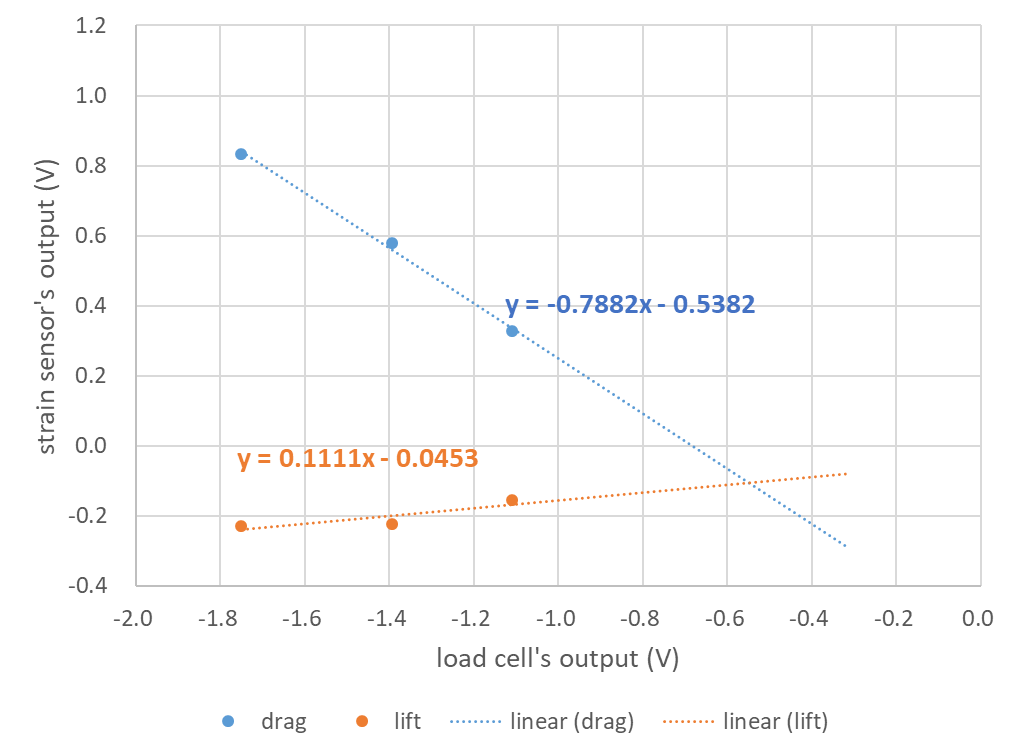
\includegraphics[width=130mm]{../images/previously_drag.png}
        \caption{previous data (drag)}
        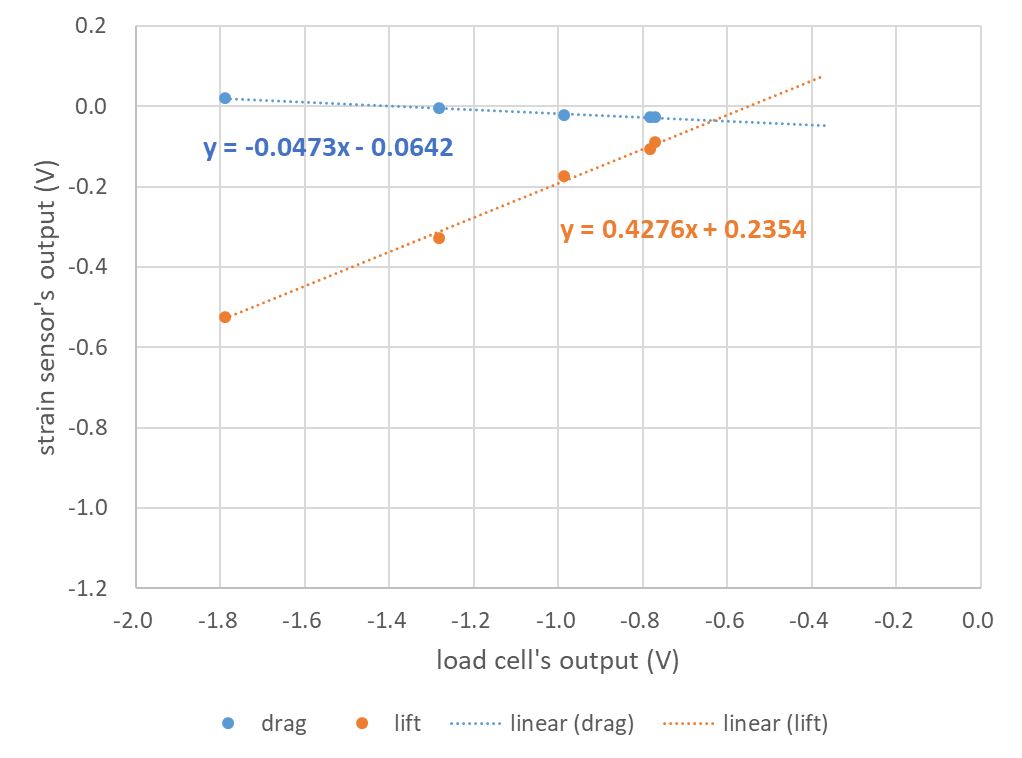
\includegraphics[width=130mm]{../images/previously_lift.png}
        \caption{previous data (lift)}
    \end{center}
\end{figure}
\newpage
\section{Range : 1k}
\begin{figure}[htbp]
    \footnotesize
    \begin{center}
        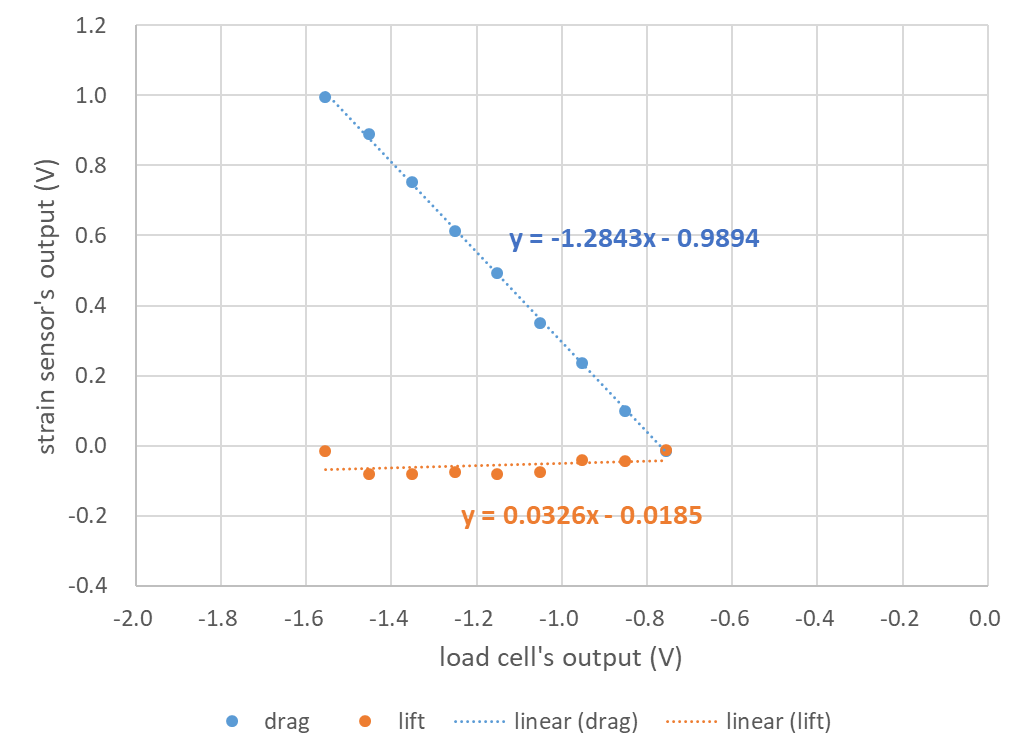
\includegraphics[width=130mm]{../images/1k_drag.png}
        \caption{range : 1k (drag)}
        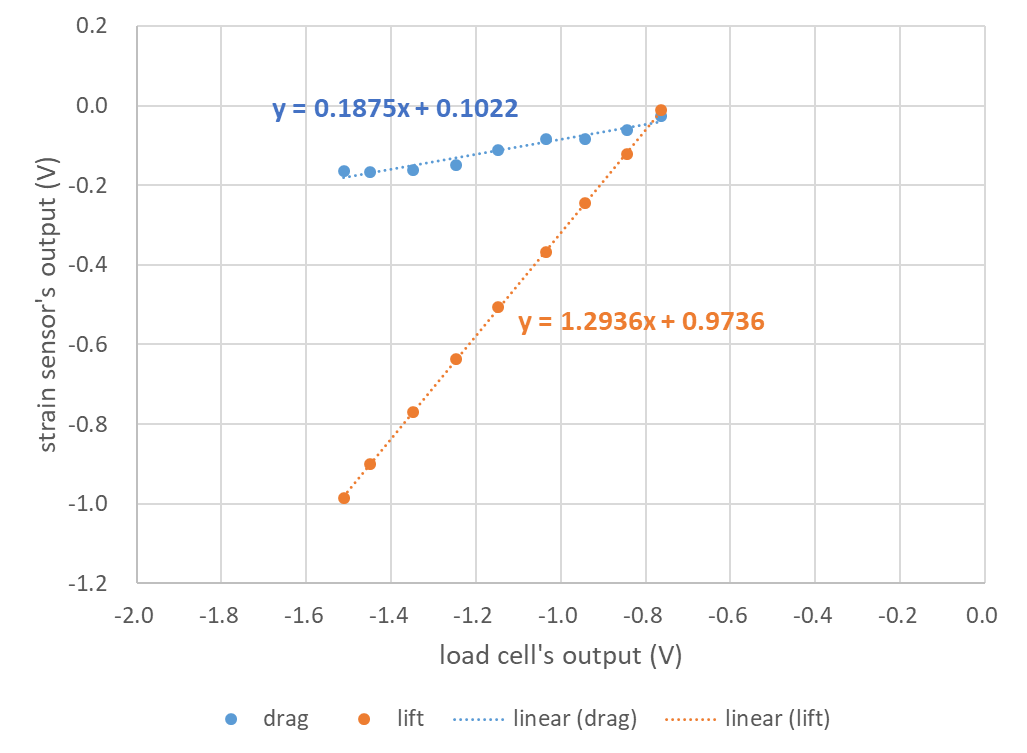
\includegraphics[width=130mm]{../images/1k_lift.png}
        \caption{range : 1k data (lift)}
    \end{center}
\end{figure}
\newpage
\section{Range : 2k}
\begin{figure}[htbp]
    \footnotesize
    \begin{center}
        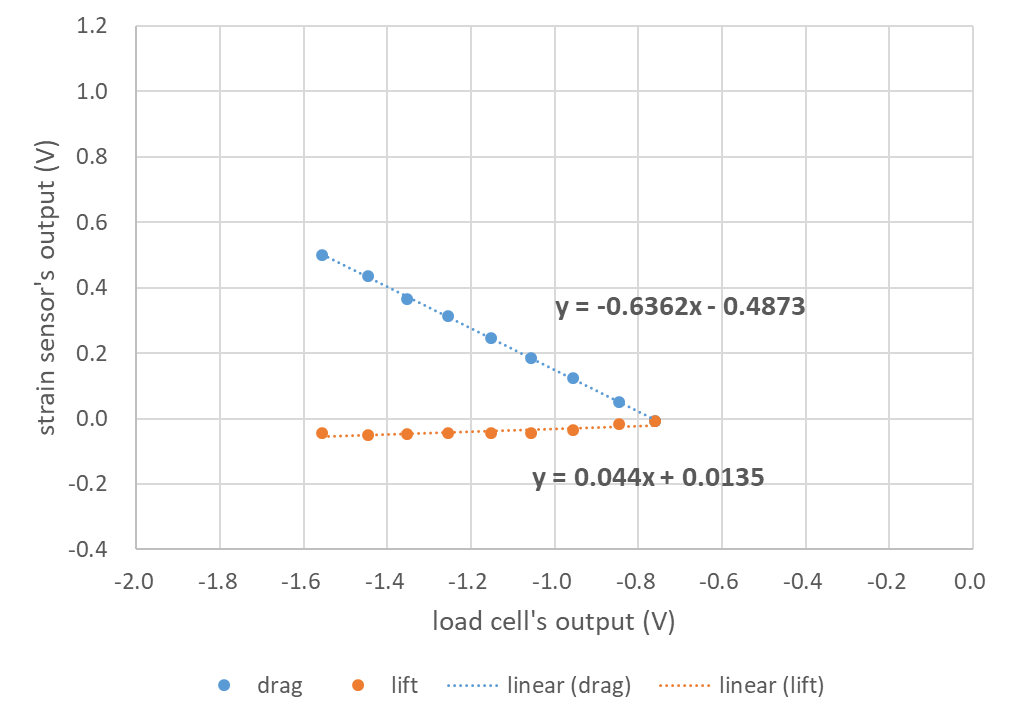
\includegraphics[width=130mm]{../images/2k_drag.png}
        \caption{range : 2k (drag)}
        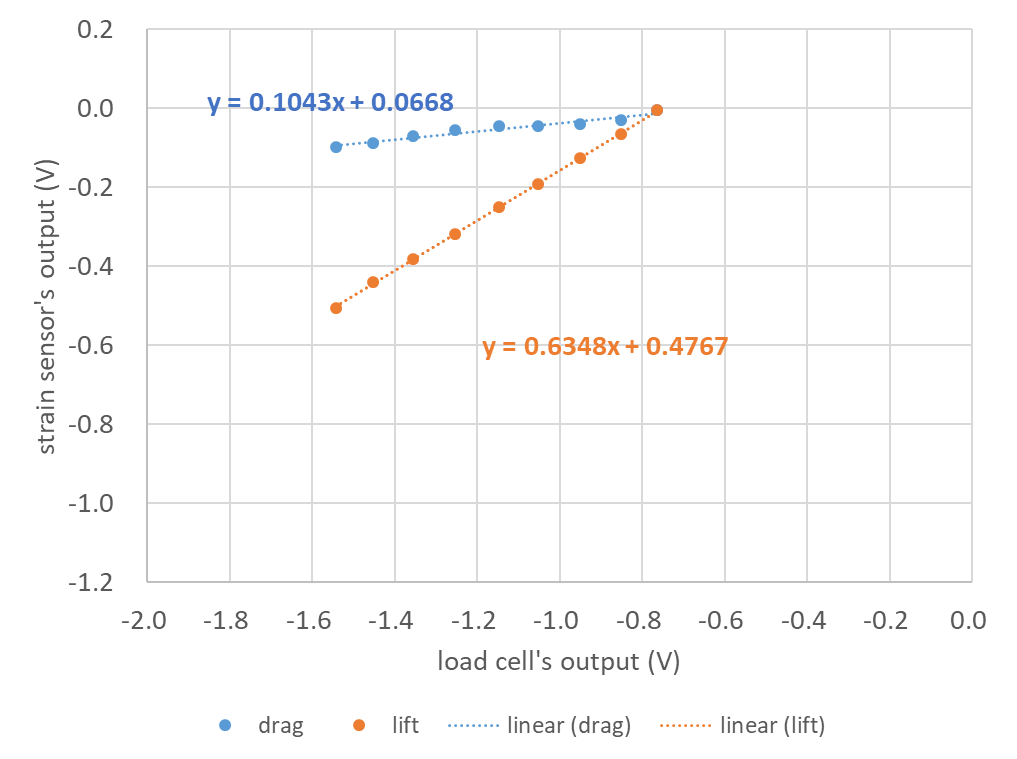
\includegraphics[width=130mm]{../images/2k_lift.png}
        \caption{range : 2k (lift)}
    \end{center}
\end{figure}
\newpage
\section{Range : 500}
\begin{figure}[htbp]
    \footnotesize
    \begin{center}
        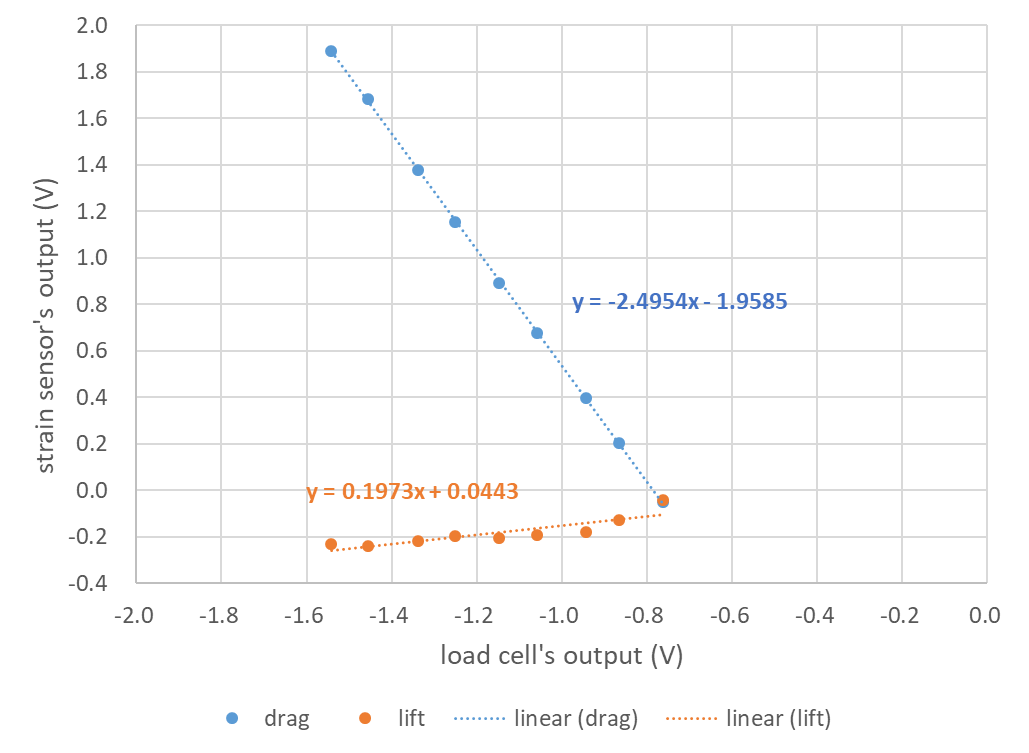
\includegraphics[width=130mm]{../images/500_drag.png}
        \caption{range : 500 (drag)}
        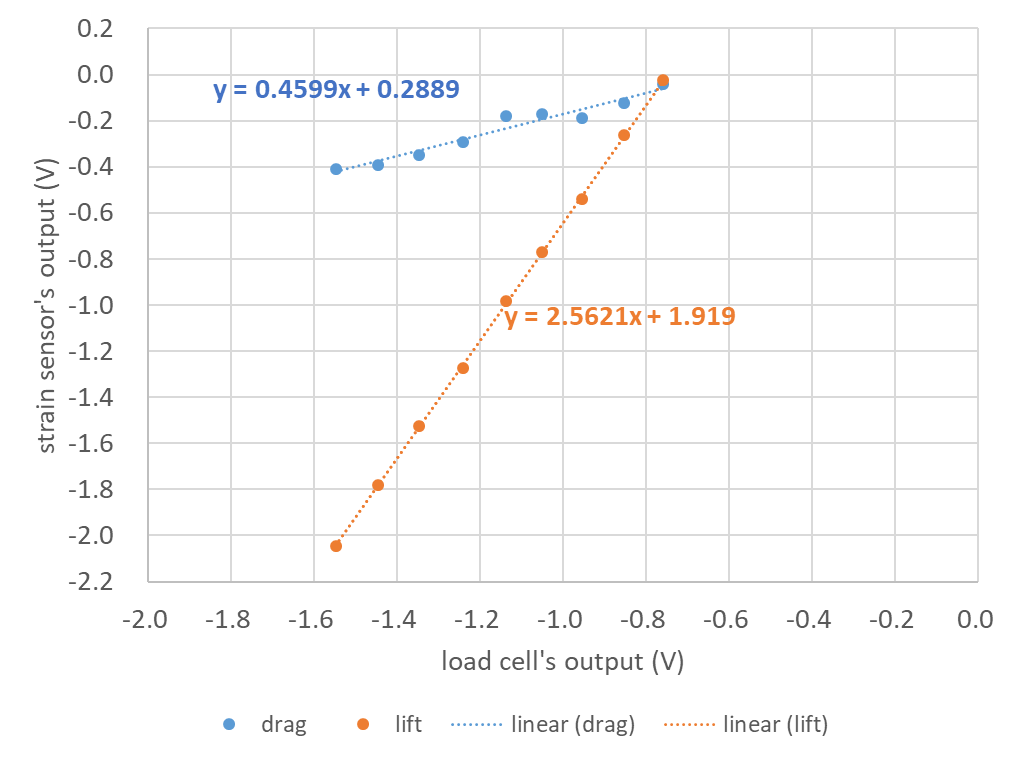
\includegraphics[width=130mm]{../images/500_lift.png}
        \caption{range : 500 (lift)}
    \end{center}
\end{figure}
\newpage
\section{Resultant force}
\begin{figure}[htbp]
    \footnotesize
    \begin{center}
        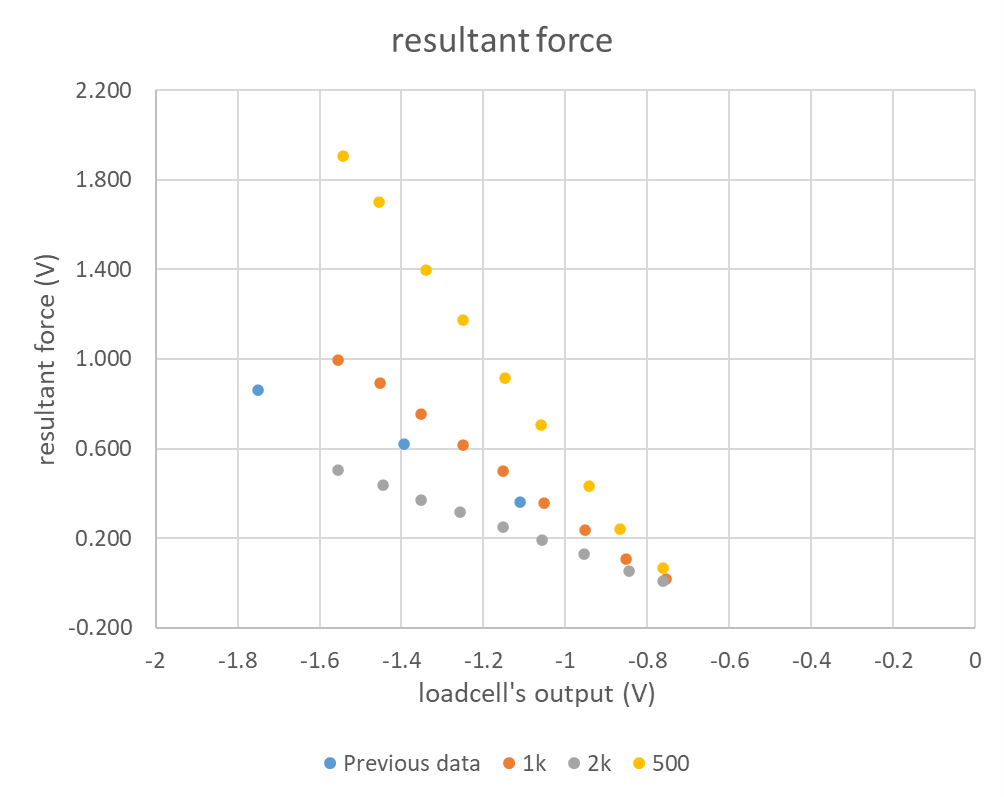
\includegraphics[width=130mm]{../images/resultantforce_drag.png}
        \caption{resultant force (drag)}
        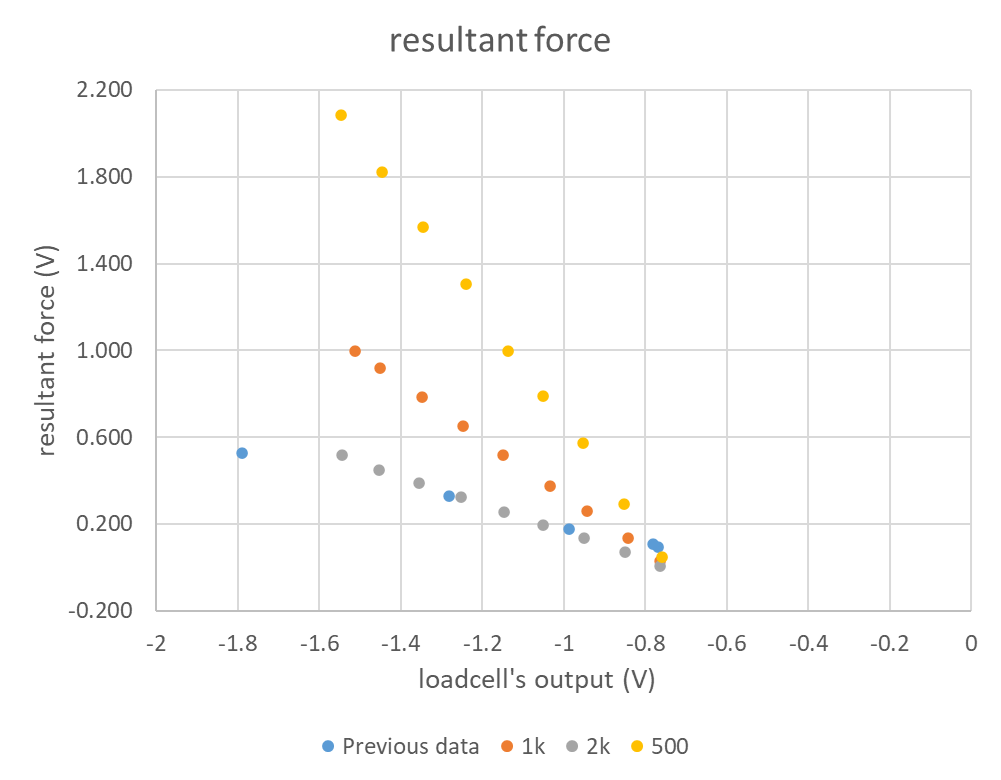
\includegraphics[width=130mm]{../images/resultantforce_lift.png}
        \caption{resultant force (lift)}
    \end{center}
\end{figure}
\end{document}